\section{Integration}


\subsection{Schemas}
Out schemas have not changed since our P2 hand-in. They are listed below.

\begin{figure}
	\centering
	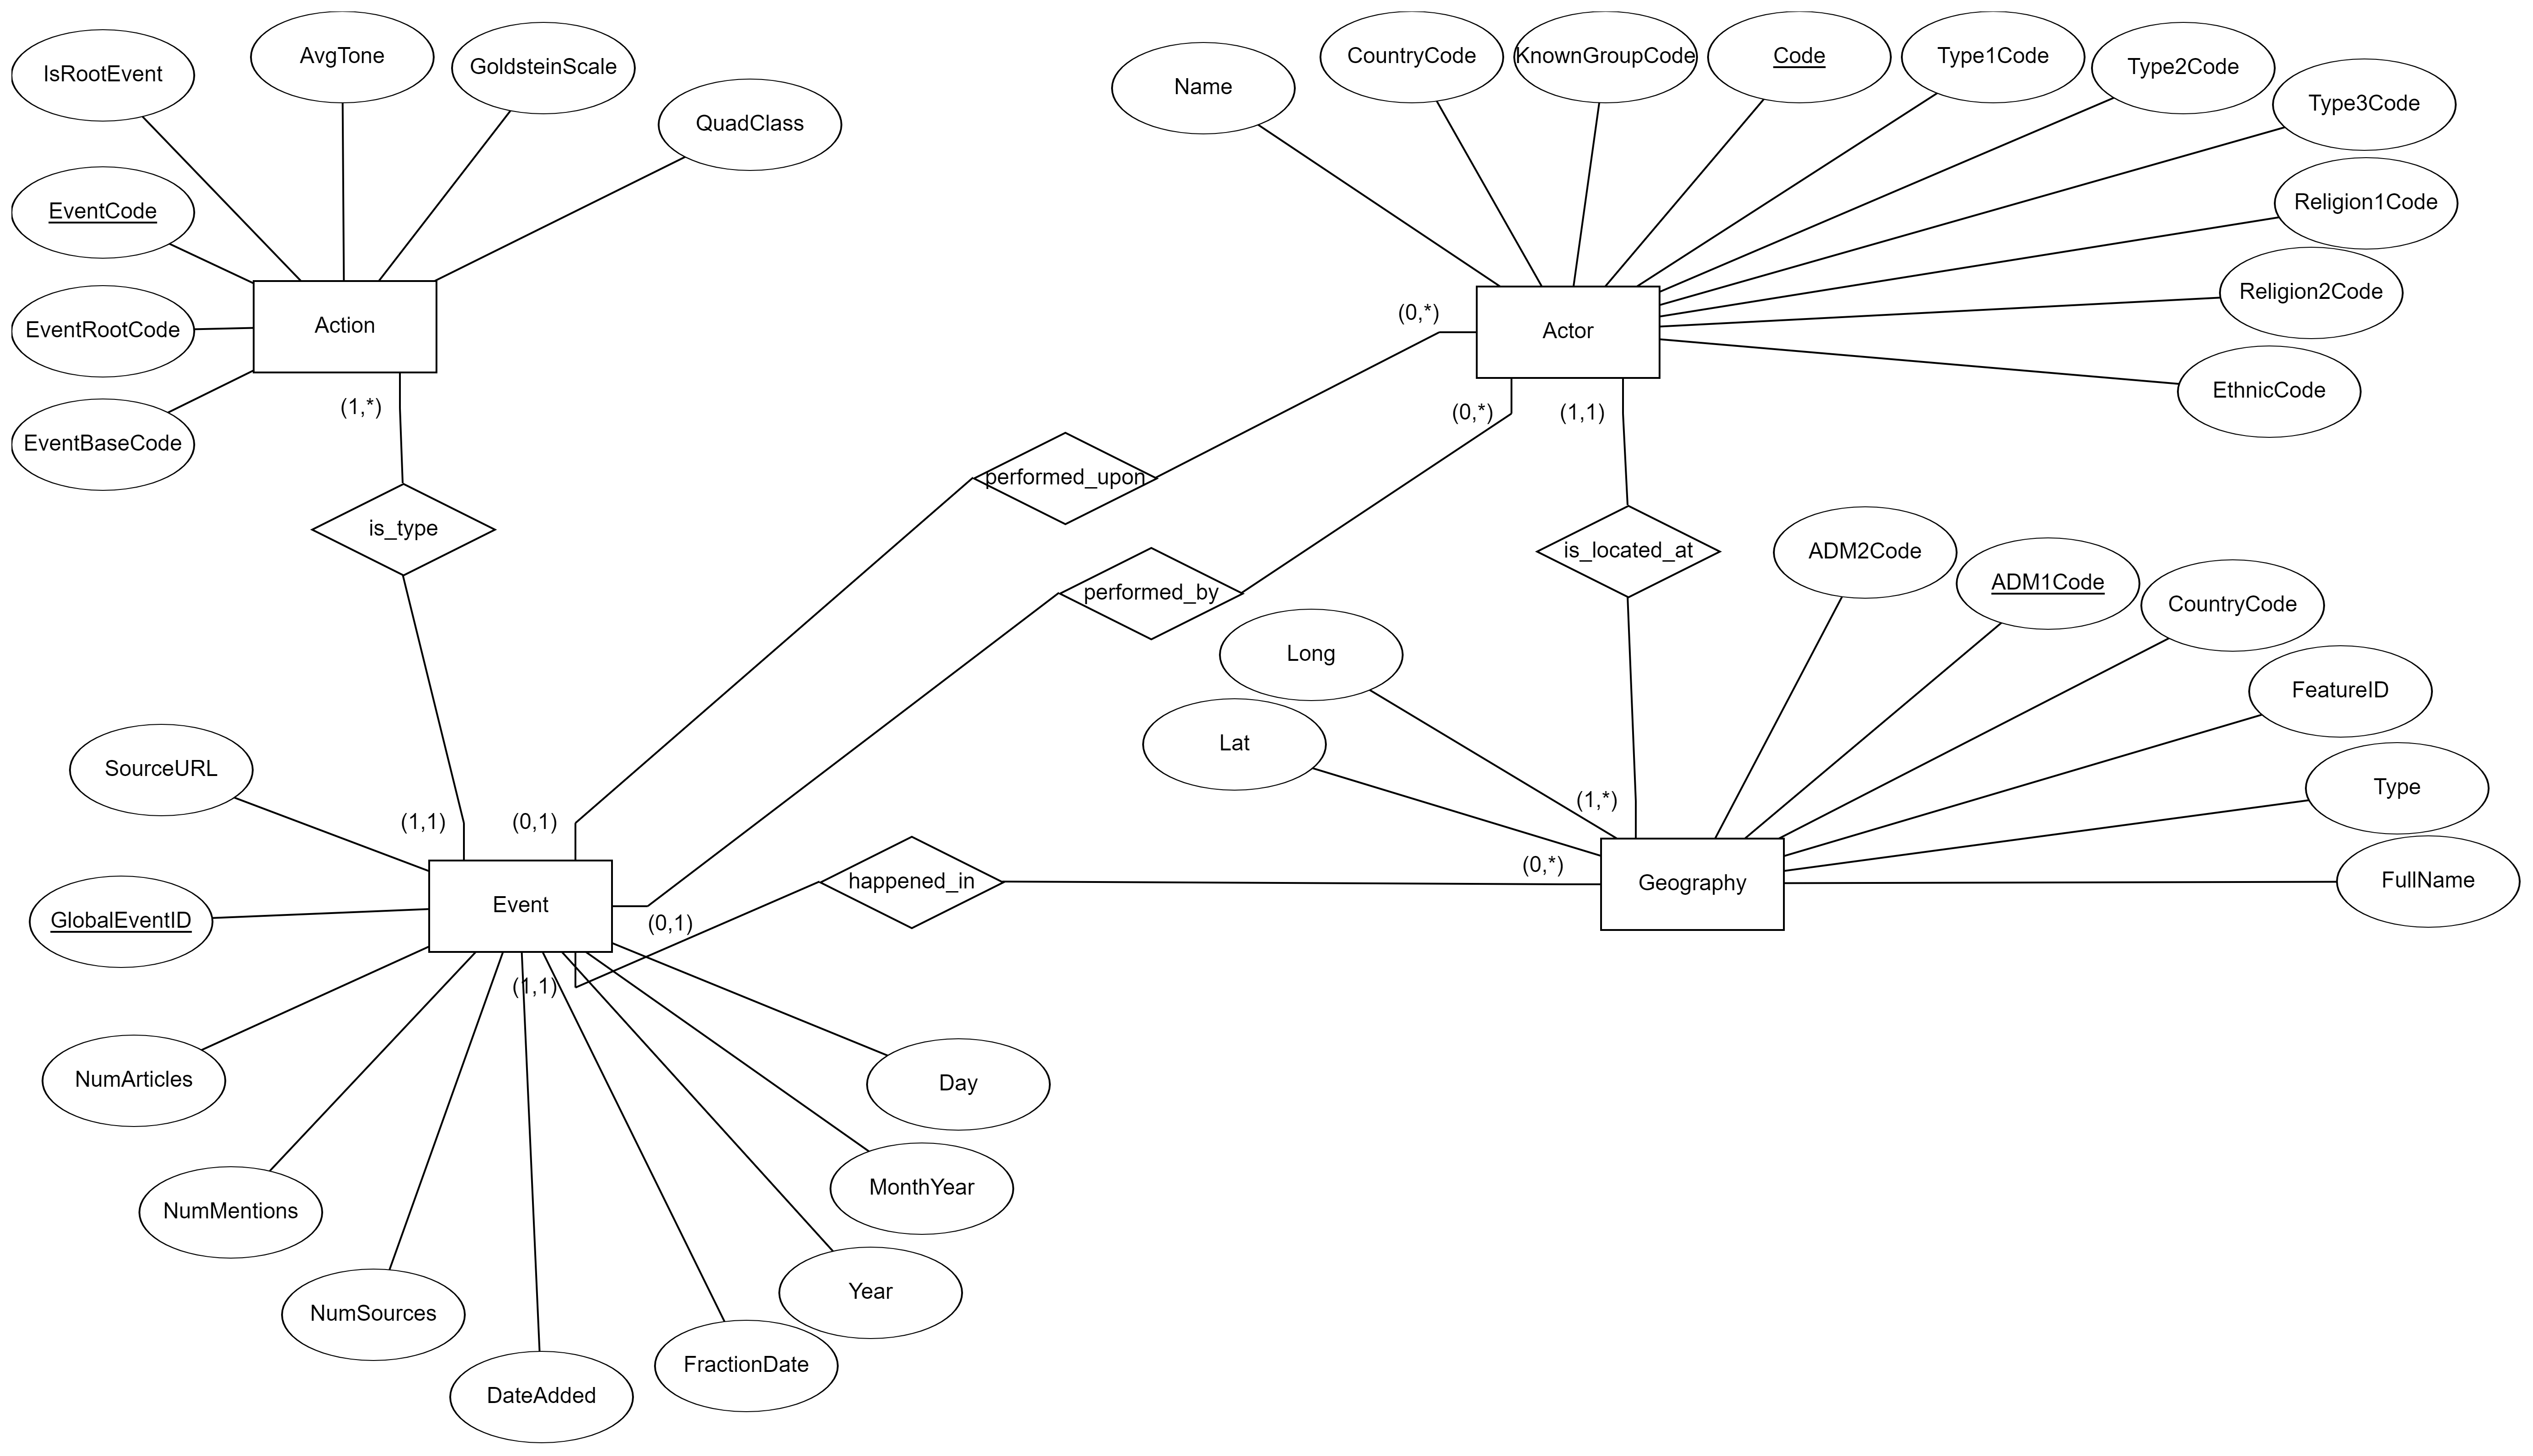
\includegraphics[scale = 0.08]{g9-gdelt}
	\caption{Our GDELT schema integration}
	\label{fig:gdelt}
\end{figure}

\begin{figure}
	\centering
	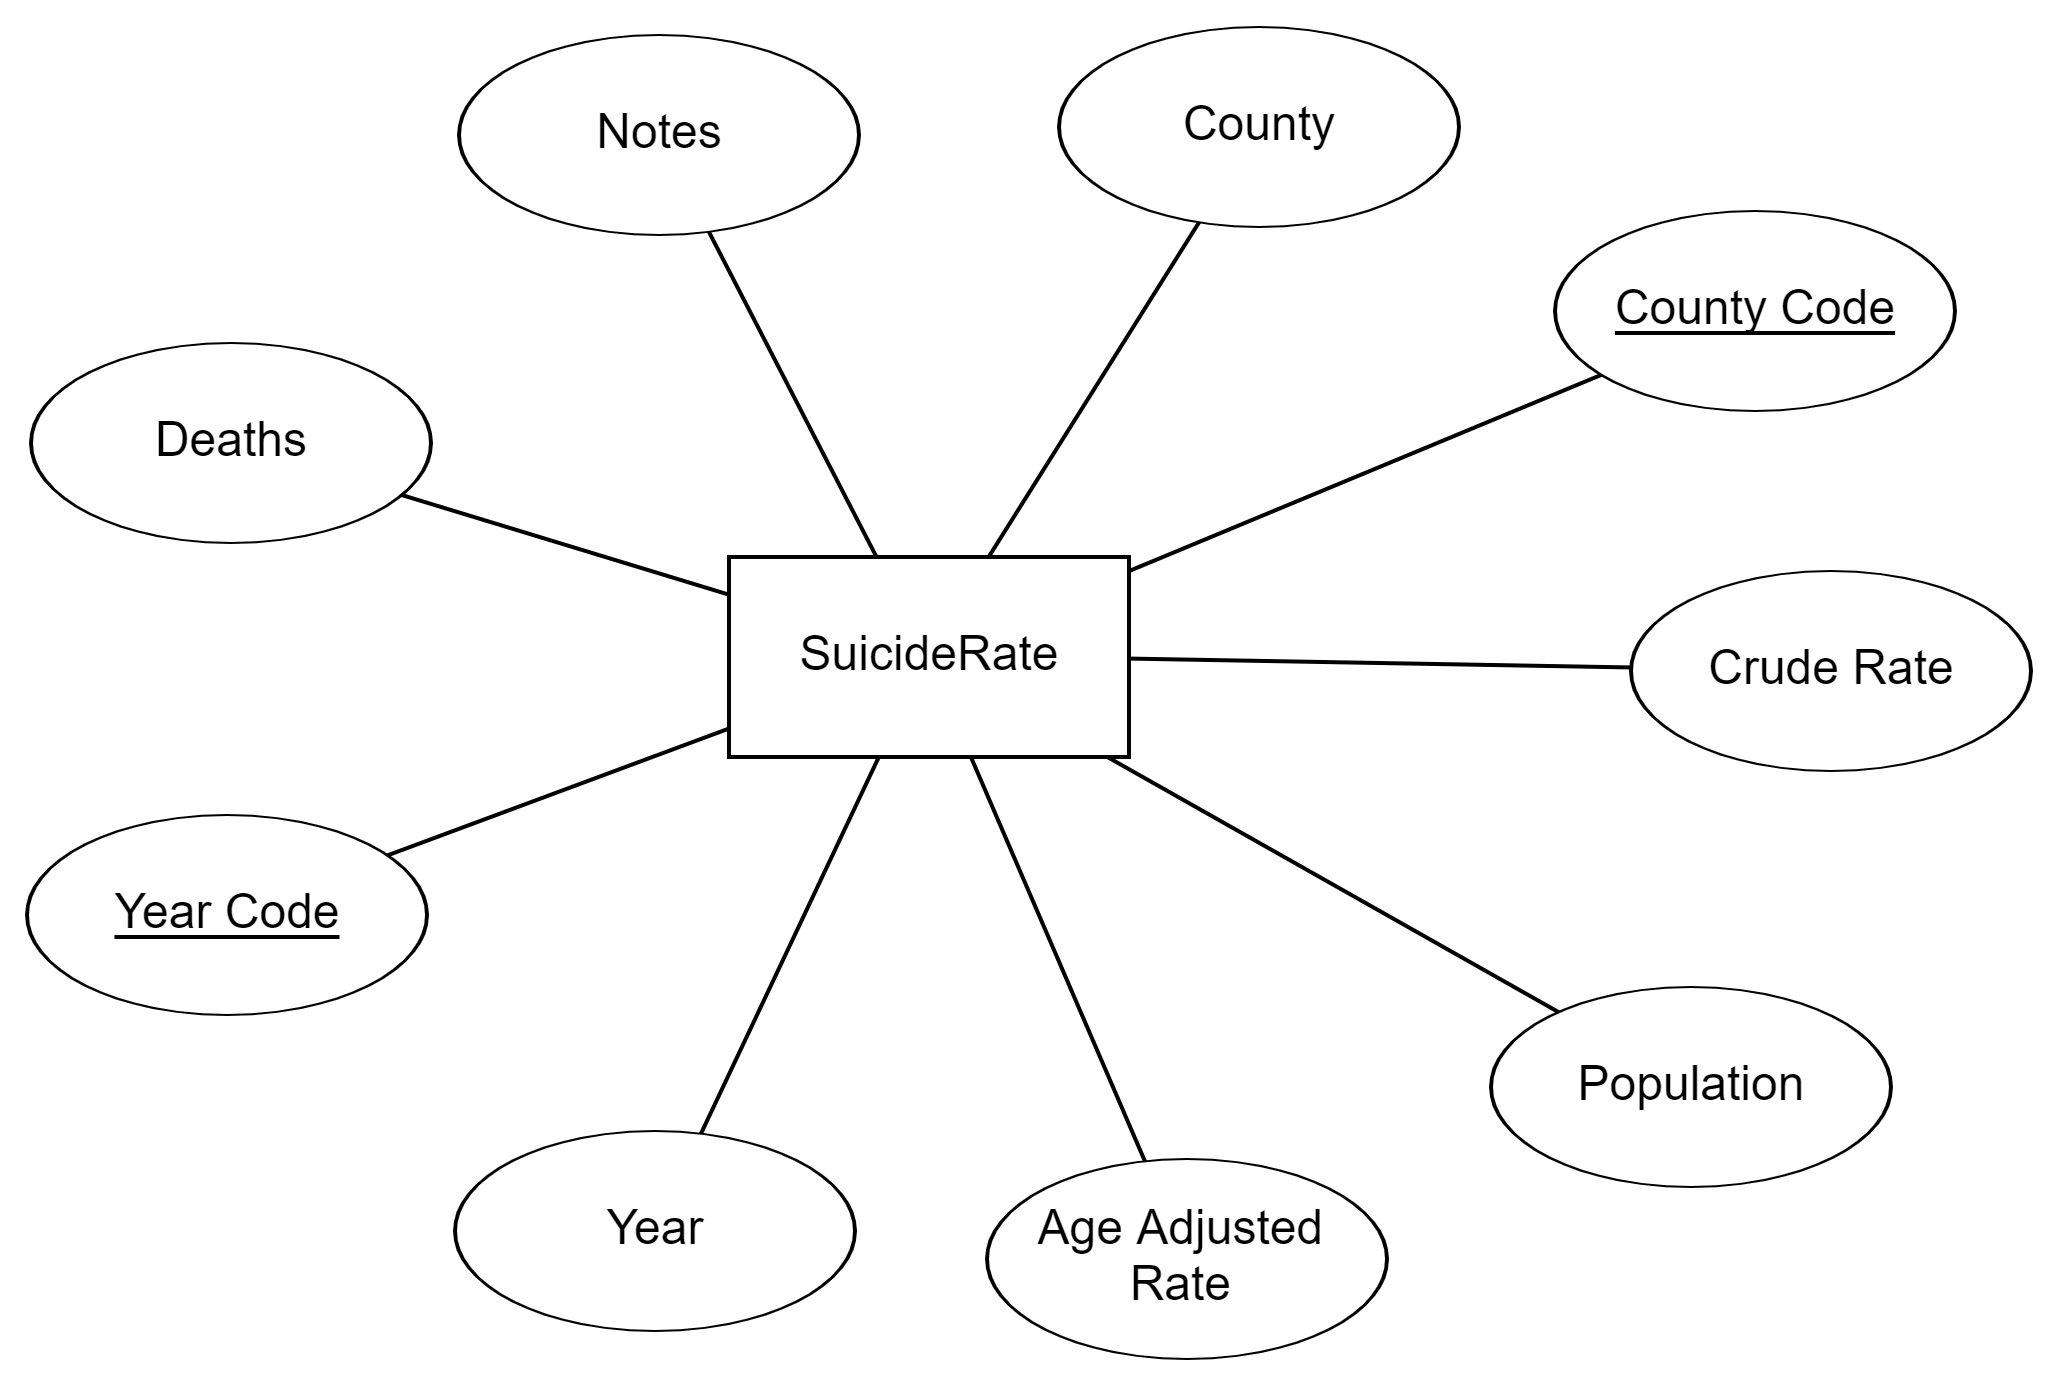
\includegraphics[scale = 0.18]{g9-suicide_rate}
	\caption{Our suicide rate schema integration}
	\label{fig:suicide_rate}
\end{figure}

\begin{figure}
	\centering
	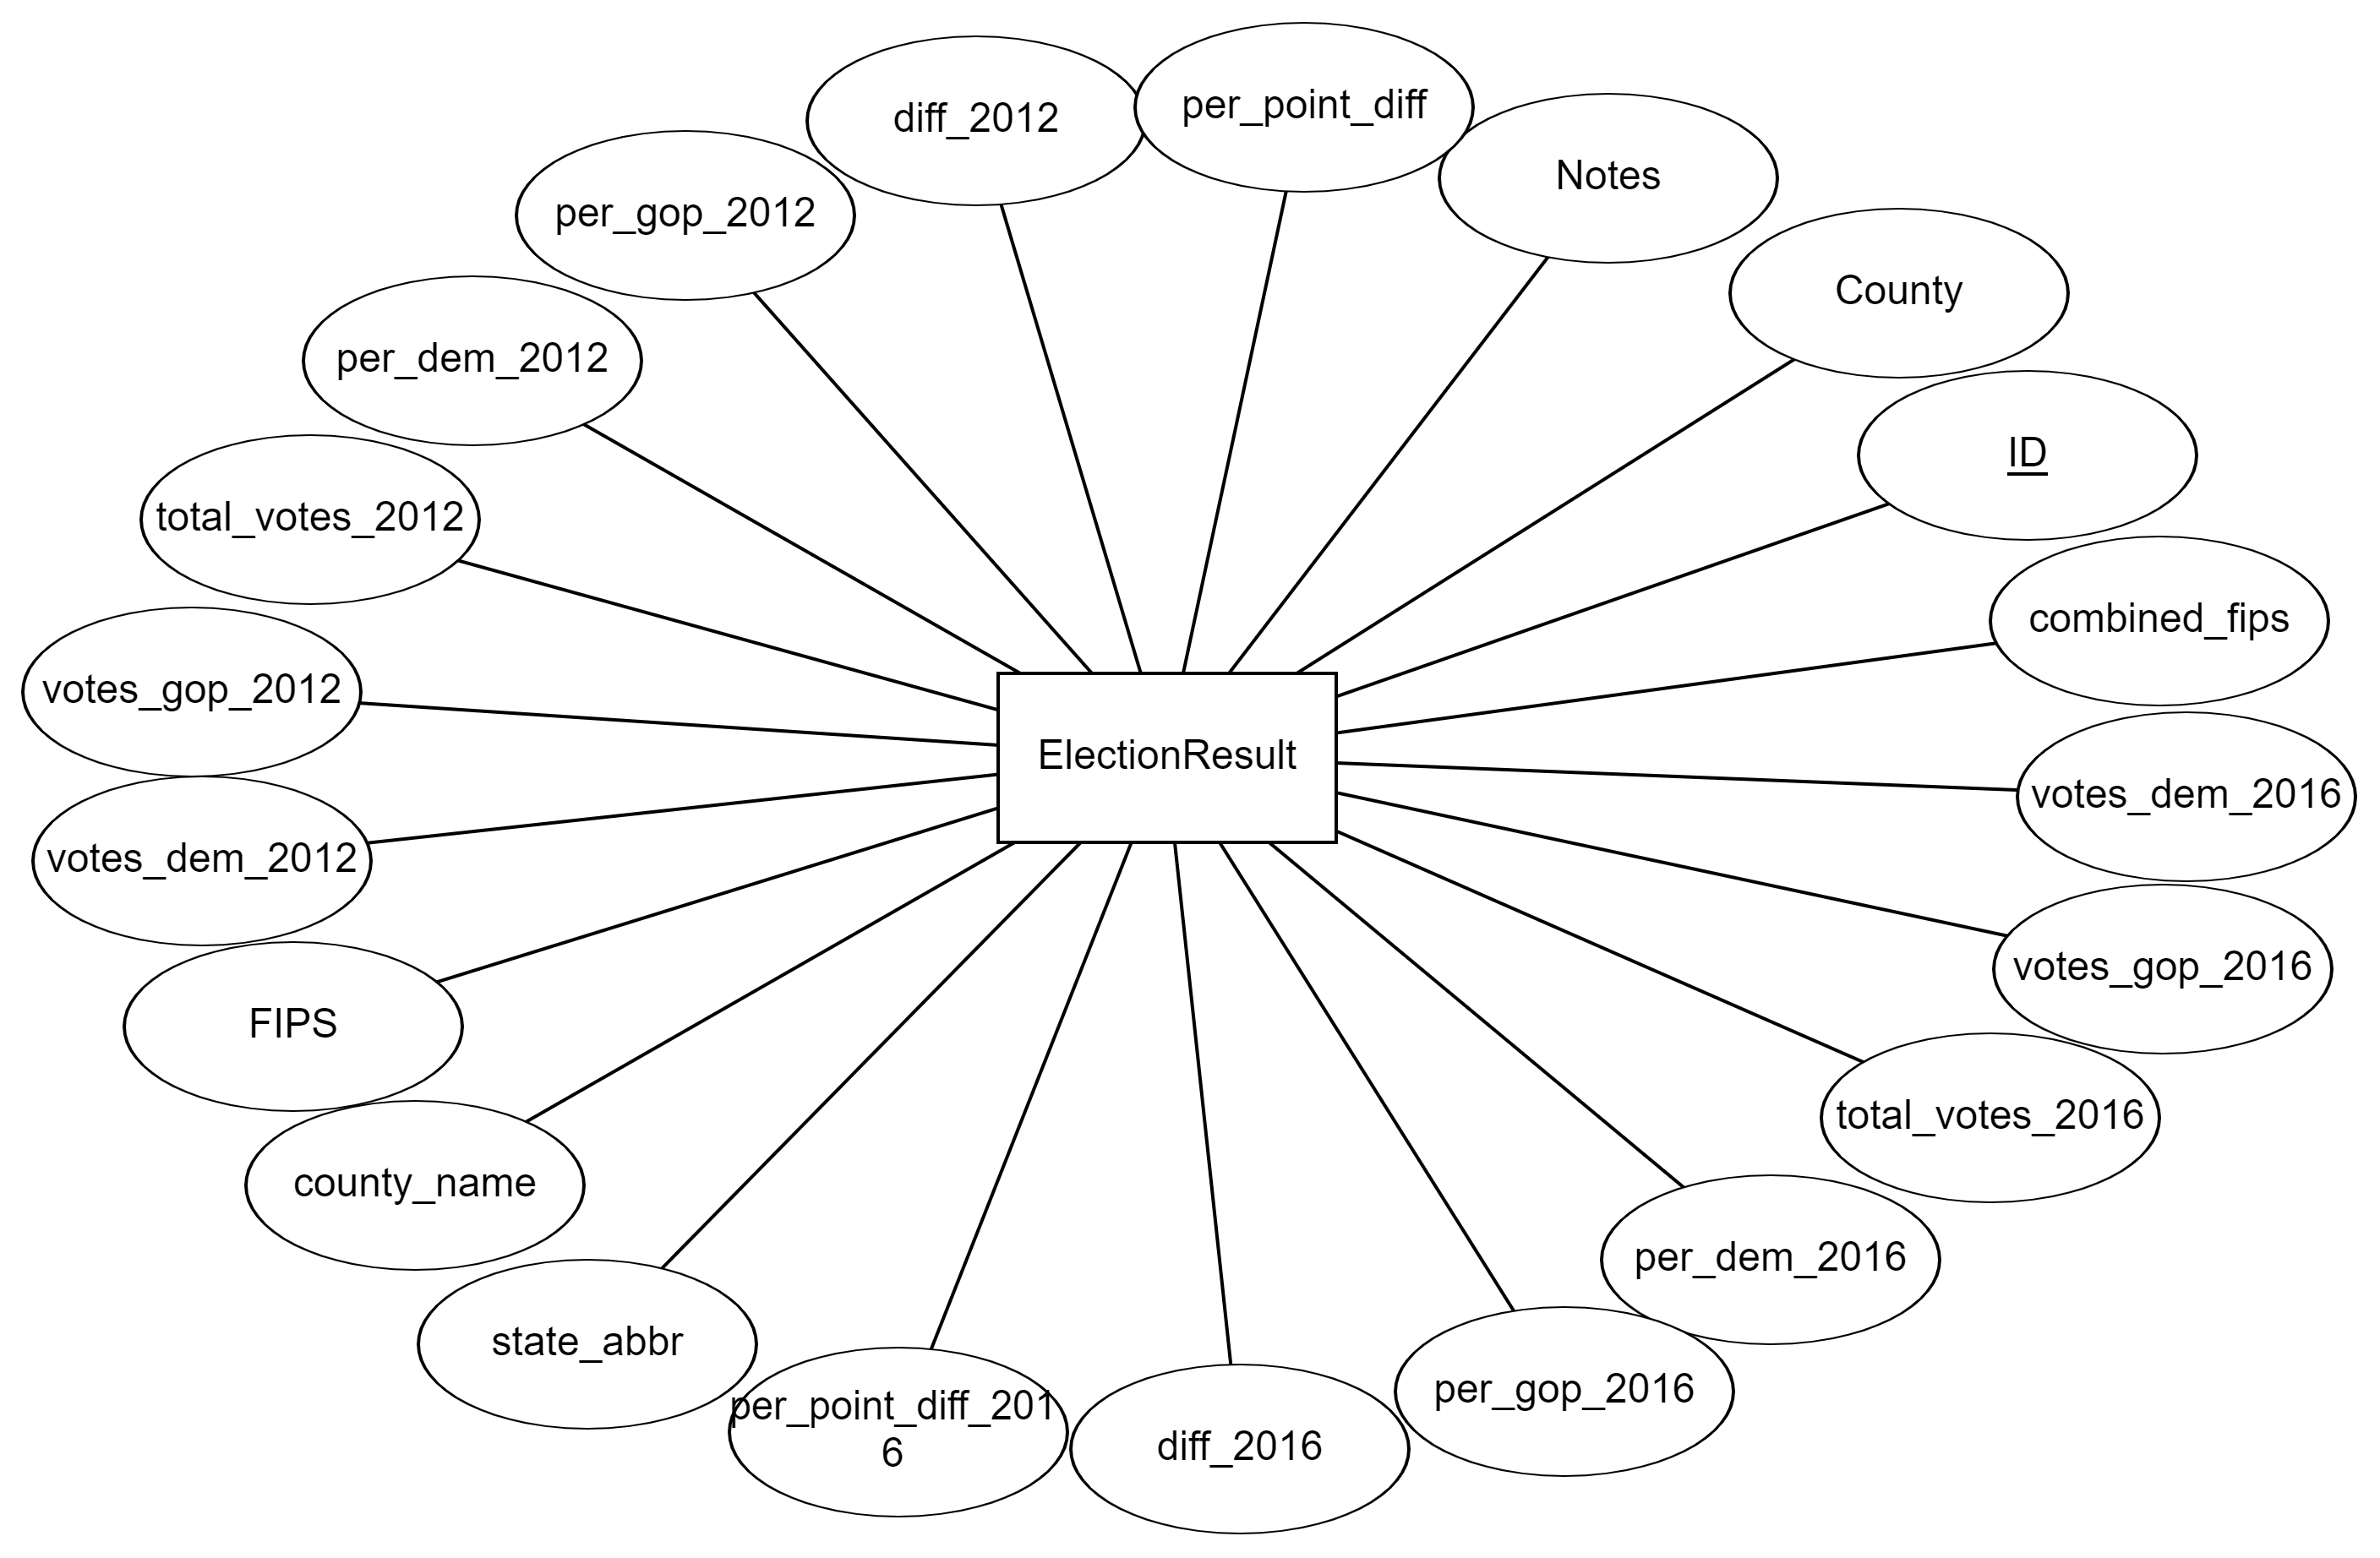
\includegraphics[scale = 0.12]{g9-election_results}
	\caption{Our election results integration}
	\label{fig:election_results}
\end{figure}

\begin{figure}
	\centering
	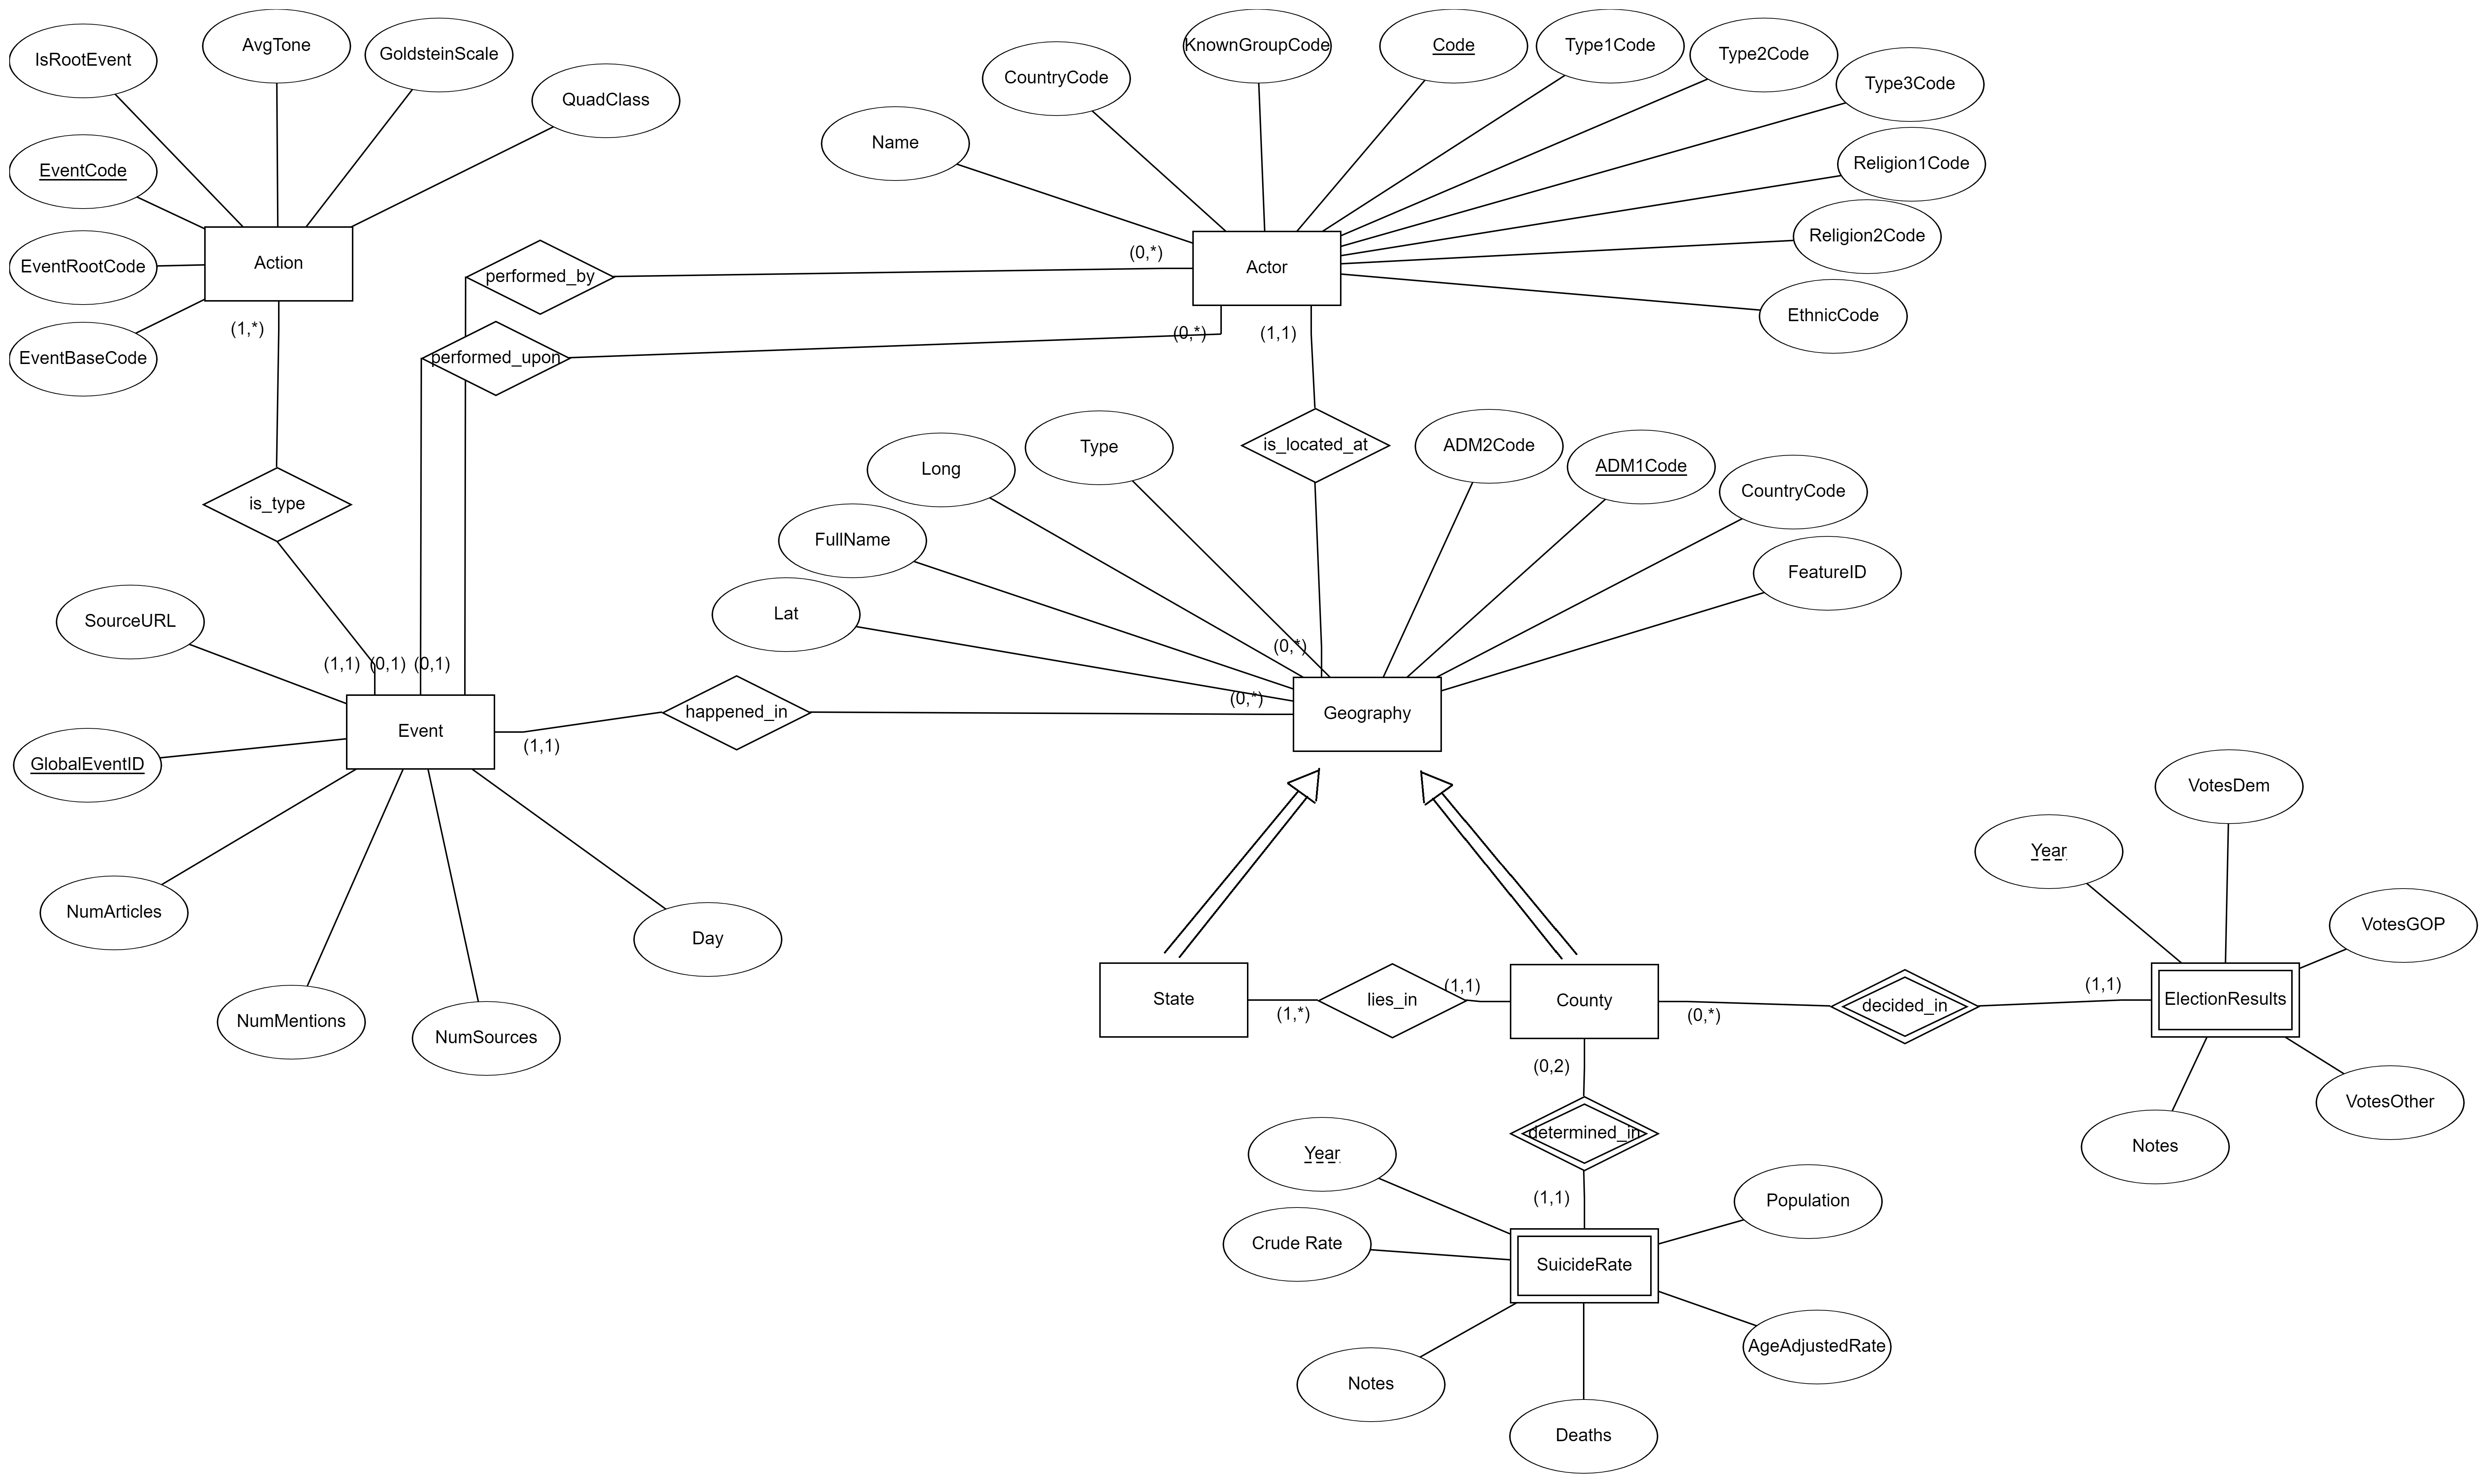
\includegraphics[scale = 0.08]{g9-all}
	\caption{Schema over the whole database}
	\label{fig:all}
\end{figure}

\subsection{Data cleaning \& normalization}
Some columns of the election results datastet and of the GDELT
dataset are redundant, e.g. in in election results percentGOP
can be computed by evaluating votesGOP * 100 / (votesGOP + votesDem)
and in in GDELT MonthYear makes the Year column irrelevant.
All of the redundant columns have not been integrated.

The GDELT data subset we use in this project consists of sixty
three thousand csv files, where each file takes somewhere between
800 KB and 1.5 MB of storage.

On our P2 hand-in we included a script
(/gdelt/download.py) that downloads and unzips each (zipped) csv file
and edits the filenames for further processing.
If a file is found to be corrupt, it is not downloaded and
the index of that file is saved in a .txt file
(/gdelt/bad\_indices.txt) for future reference.

A problem occurs when populating the ElectionResult table when
the geoId code of a county on the Election dataset does not
match any of the County-table's (already fully populated) goidIds.
In that case the corresponding
row is simply skipped and also printed to STDOUT for reference
(this only happens for Alaska).
